\documentclass[12pt,a4paper]{article}

\usepackage{inputenc}
\usepackage[english]{babel}
\usepackage[T1]{fontenc}
\usepackage{amsmath}
\usepackage{amsfonts}
\usepackage{amssymb}
\usepackage{graphicx}
\usepackage{epstopdf}
\usepackage{url}
\usepackage{cite}
\usepackage{color}
\usepackage{ifthen}
\usepackage[top=1cm,bottom=0.5cm,right=1cm,left=1cm]{geometry}
\usepackage{algorithm}
\usepackage{algpseudocode}
\usepackage{algorithmicx}


%\floatname{algorithm}{Procedure}
\renewcommand{\algorithmicrequire}{\textbf{Input:}}
\renewcommand{\algorithmicensure}{\textbf{Output:}}

%N�cessite les packages "color" et "ifthen"
\makeatletter
\newcommand{\sectioncolor}{blue} %Couleur titre de section
\newcommand{\ssectioncolor}{cyan} %Couleur titre de sous-section
\newcommand{\sssectioncolor}{magenta} %Couleur titre de sous-sous-section
%
%Coloration des titres
%---------------------
\renewcommand{\section}{%Commande d�finie dans le fichier article.cls
    \@startsection%
    {section}%
    {1}%
    {0pt}%
    {-3.5ex plus -1ex minus -.2ex}%
    {2.3ex plus.2ex}%
    {\color{\sectioncolor}\normalfont\Large\bfseries\centering}} %Aspect du titre
\renewcommand\subsection{%
    \@startsection{subsection}{2}{\z@}%
    {-3.25ex\@plus -1ex \@minus -.2ex}%
    {1.5ex \@plus .2ex}%
    {\color{\ssectioncolor}\normalfont\large\bfseries\centering}}
\renewcommand\subsubsection{%
    \@startsection{subsubsection}{3}{\z@}%
    {-3.25ex\@plus -1ex \@minus -.2ex}%
    {1.5ex \@plus .2ex}%
    {\color{\sssectioncolor}\normalfont\normalsize\bfseries\centering}}
%
%Coloration de la table des mati�res
%-----------------------------------
\renewcommand{\addcontentsline}[3]{%Commande d�finie dans le fichier latex.ltx
  \ifthenelse{\equal{#2}{section}}{%
    \addtocontents{#1}{\protect\contentsline{#2}{\color{\sectioncolor}#3}{%
        \color{\sectioncolor}\thepage}}}{% #2=titre, #3=num. de page
        \ifthenelse{\equal{#2}{subsection}}{%
            \addtocontents{#1}{\protect\contentsline{#2}{\color{\ssectioncolor}#3}{%
                \color{\ssectioncolor}\thepage}}}{%
                \ifthenelse{\equal{#2}{subsubsection}}{%
                    \addtocontents{#1}{\protect\contentsline{#2}{\color{\sssectioncolor}#3}{%
                        \color{\sssectioncolor}\thepage}}}{}}}}
\makeatother
%Coloration en noir du titre "Table des mati�res"
\let\cn=\contentsname
\renewcommand{\contentsname}{\normalcolor\cn}


\pagestyle{empty}




\begin{document}

%%%%%%%%%%%%%%%%%%%%%% FRAME 1 %%%%%%%%%%%%%%%%%%%%%%

\vspace{2cm}
\begin{center}
\Huge \color{blue}{\textbf{Scene Text Recognition}} \color{black}\\
\large Vincent BODIN \& Thomas MOREAU
\end{center}
\hrulefill
\normalsize
\vspace{2cm}


\begin{abstract}
\emph{Scene text recognition refers to finding automatic ways of extracting text in pictures of every day life. As computer vision is more and more successful, scene text recognition has naturally become a significant issue nowadays. Unlike OCR which is more or less well understood and implemented, scene text recognition still needs many improvement to be considered as a powerful tool. We implemented paper \cite{Mis} that explains how to extract words efficiently. A graphical model is introduced inside, with the creation of graph represented possible detected words, and algorithm TRW-S \cite{Kol} is used to extract the optimal one.}
\end{abstract}

\vspace{2cm}

\section{Introduction}

Our task is to extract from a picture the underlying text, and determine what word is being written. It mainly requires two steps:
\begin{description}
\item[Step 1:] We have to detect all the possible characters in the picture. It is very important not to miss one so that leads us to a very flexible criterion of selection. 

\item[Step 2:] Among all those possible characters, try to find those which really are ones, and construct a word from them. 
\end{description}
In this project we will essentially be interested in the second step of the project, the first one being implemented in \emph{Object Recognition and Computer Vision} course.


\newpage
%%%%%%%%%%%%%%%%%%%%%% FRAME 2 %%%%%%%%%%%%%%%%%%%%%%


\begin{figure}[!ht]
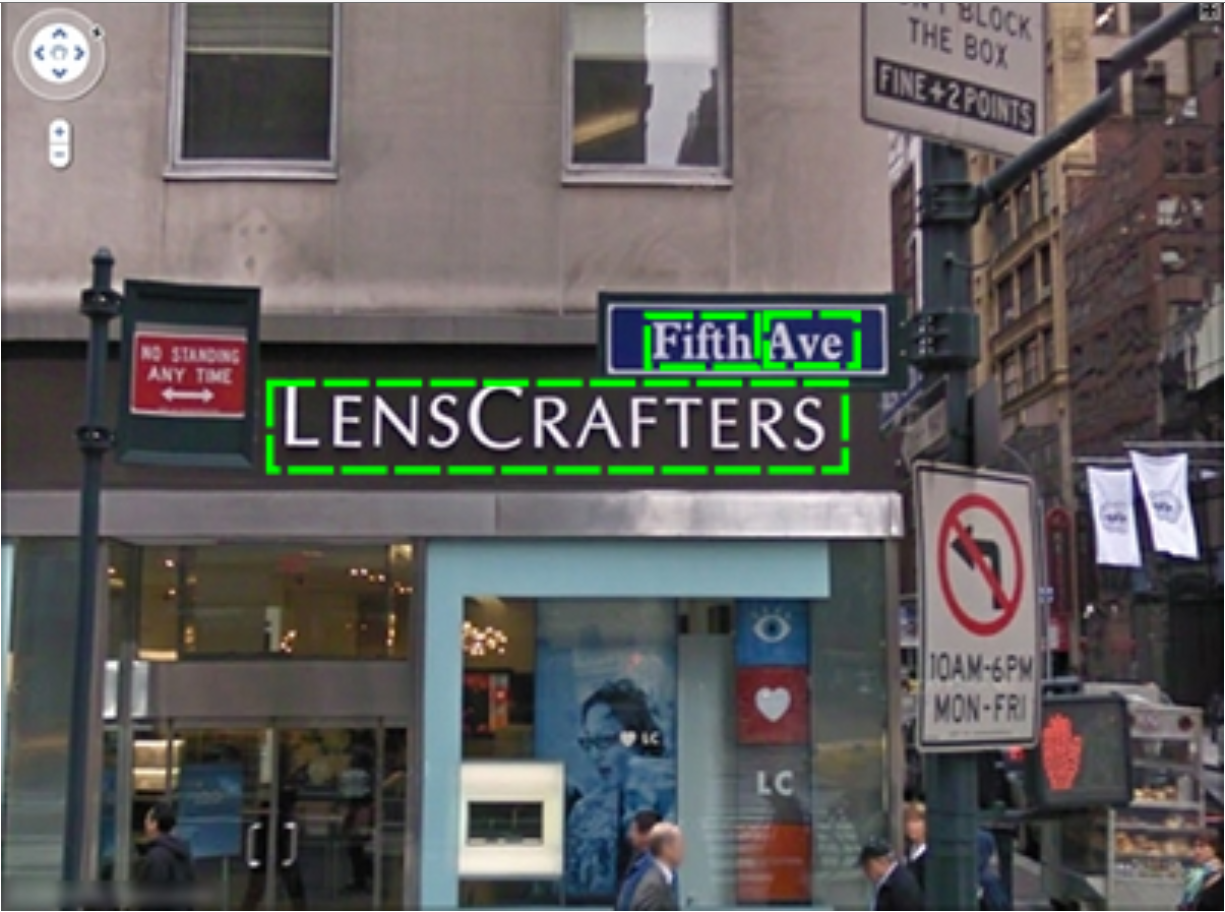
\includegraphics[width=\columnwidth]{figures/intro.png}%
\caption{Task}%
\label{}%
\end{figure}









%%%%%%%%%%%%%%%%%%%%%% FRAME 3 %%%%%%%%%%%%%%%%%%%%%%


\section{The graphical model construction}

\subsection{Learning characters and words}

\begin{description}
\item[Learning characters. ] We need to build classifiers for each character to recognize them in natural pictures. 
	\begin{itemize}
		\item Use a database to identify characters: ICDAR 2003 \cite{ICDARchar}, Chars74K \cite{Char74K};
		\item extract features: Histogram Of Gradient (HOG) \cite{Dal2005}. They extract the information of a patch by computing the gradient on bins of sizes $4\times 4$, saved in an histogram of 12 orientations;
		\item build $K$ SVMs ($K$ is the number of classes, 62) with RBF Kernel, Fig.(\ref{RBFKernel}):
		\begin{equation}
		\exp(-\gamma |x-x'|^2), \gamma > 0
		\label{eq:}
		\end{equation}
		method one-versus-all, we used a Python librairy scikit-learn \cite{scikit}: two parameters $\gamma$ and regularization $C$ optimized by cross-validation -> test error without optimization $25\%$, with optimization $16\%$.
	\end{itemize}
	\begin{figure}[ht!]
	\centering
	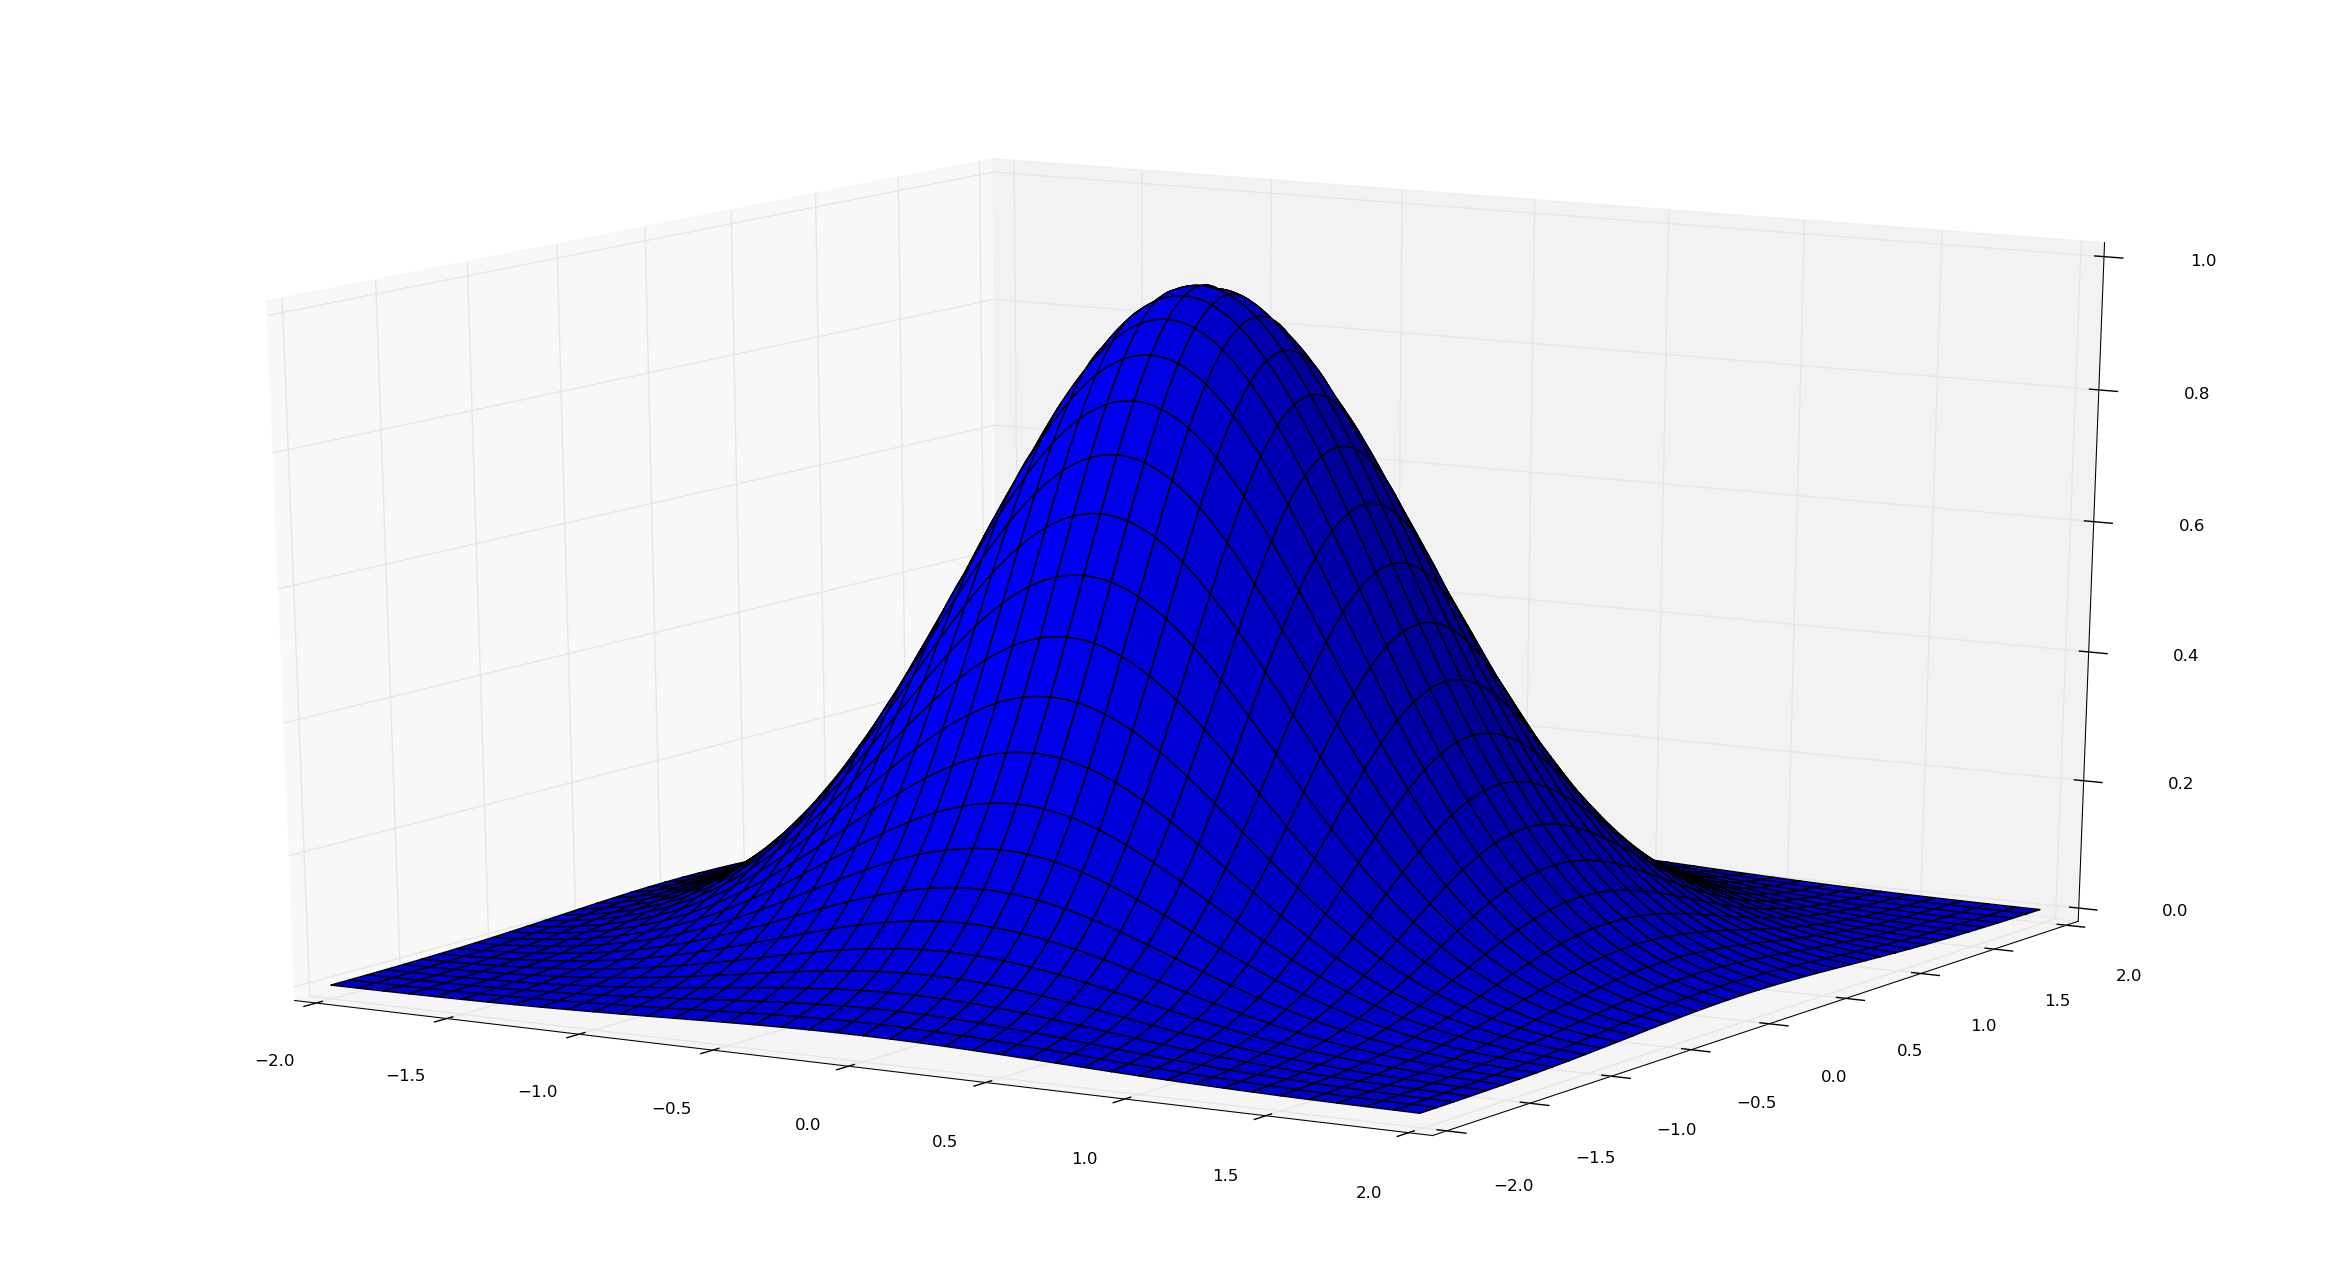
\includegraphics[width=10cm]{figures/blob.png}%
	\caption{RBF Kernel}%
	\label{RBFKernel}%
	\end{figure}
	
\item[Learning words. ] We have to build a prior lexicon that contains how characters interact to create words, for this:
	\begin{itemize}
		\item Load a database of words \cite{ICDARword};
		\item count for each pair of characters $(c_i,c_j)$ their frequency of occurrence $p(c_i,c_j)$ in the database (bi-gram model);
	\end{itemize}
This frequency of occurrences will be used to penalize through an energy term the pair of words that are rare in the dictionary (\emph{e.g.} 'xz').
\end{description}









\newpage
%%%%%%%%%%%%%%%%%%%%%% FRAME 4 %%%%%%%%%%%%%%%%%%%%%%

\subsection{Character detection: sliding windows}

The first task is to detect all possible characters in the image, this is done through the sliding windows algorithm:

\begin{algorithm}
\caption{Sliding Window scanning}
\label{algo1}
\begin{algorithmic}
\Require Image
\Ensure l list of characters

\State l = [ ]; 
\For {all windows in Image}
	\State $p \leftarrow$ svm.predict\_proba
	\State GS $\leftarrow \max_c p(c|\phi_i) \exp\left( - \frac{(a_i - \mu_{a_j})^2}{2\sigma_{a_j}^2} \right)$
		\If {GS > 0.1}
		\State l.append(window) 
	\EndIf
\EndFor
\end{algorithmic}
\end{algorithm}

We did not specify in here the grid we took for the width and the height of the windows: for the moment, to avoid too many detection, we rather tune it by ourselves, giving a range close to the actual size of the letters in the image. 

\begin{algorithm}
\caption{Non-Maximum Suppresion (NMS)}
\label{algo2}
\begin{algorithmic}
\Require $l$ list of windows, $c$ character with maximum probability for each window, threshold
\Ensure $l_p$ pruned list

\While {$l$ is not empty}
	\State $w_1, c_1$ pair of characters in l with highest probability
	\State $m = [w]$
	\For {$w_2,c_2$ in $l,c$}
		\If {criterion > threshold and $c_1 == c_2$}
			m.append($w_2$)
		\EndIf
	\EndFor
	\State $l_p$.append(mean($m$),$p$)
\EndWhile
\end{algorithmic}
\end{algorithm}


%\begin{algorithm}[H]
	%\SetAlgoLined % For previous releases [?]
	%\KwData{this text}
	%\KwResult{how to write algorithm with \LaTeX2e }
	%initialization\;
	%\text{l} = []\;
	%\For{all windows in Image}{
		%p \leftarrow \text{svm.predict_proba} \;
		%\text{GS} \leftarrow \text{formule} \;
		%\If{GS>0}{
			%l.append(window)
		%}
	%}
	%\caption{Sliding windows}
%\end{algorithm}








\newpage
%%%%%%%%%%%%%%%%%%%%%% FRAME 5 %%%%%%%%%%%%%%%%%%%%%%











\newpage
%%%%%%%%%%%%%%%%%%%%%% FRAME 6 %%%%%%%%%%%%%%%%%%%%%%













\newpage
%%%%%%%%%%%%%%%%%%%%%% FRAME 7 %%%%%%%%%%%%%%%%%%%%%%












\newpage
%%%%%%%%%%%%%%%%%%%%%% FRAME 8 %%%%%%%%%%%%%%%%%%%%%%











\bibliographystyle{unsrt}
\bibliography{biblio}



\end{document}